\documentclass{beamer}

\mode<presentation>
{
  \usetheme{Darmstadt}      % or try Darmstadt, Madrid, Warsaw, ...
  \usecolortheme{default} % or try albatross, beaver, crane, ...
  \usefonttheme{serif}  % or try serif, structurebold, ...
  \setbeamertemplate{navigation symbols}{}
  \setbeamertemplate{caption}[numbered]
} 
 
\usepackage[utf8]{inputenc}
\usepackage[]{algorithm2e}

%Information to be included in the title page:
\title{Nat-Sci II Presentation: \\
Editing of Pig DNA May Lead to More Organs for People}
\author{YD Choi, Amy Jung, Vaughn Tajirian, Katie Westerlund }
\institute{New York University}
 
\begin{document}
 
\frame{\titlepage} 

\begin{frame}
\frametitle{The Article under Investigation}
\begin{itemize} 
\item ``Editing of Pig DNA May Lead to More Organs for People,`` appeared in
New York times Science section (10/15/15). Written by Carl Zimmer.
\end{itemize}
\begin{figure}[h!]
  \centering
    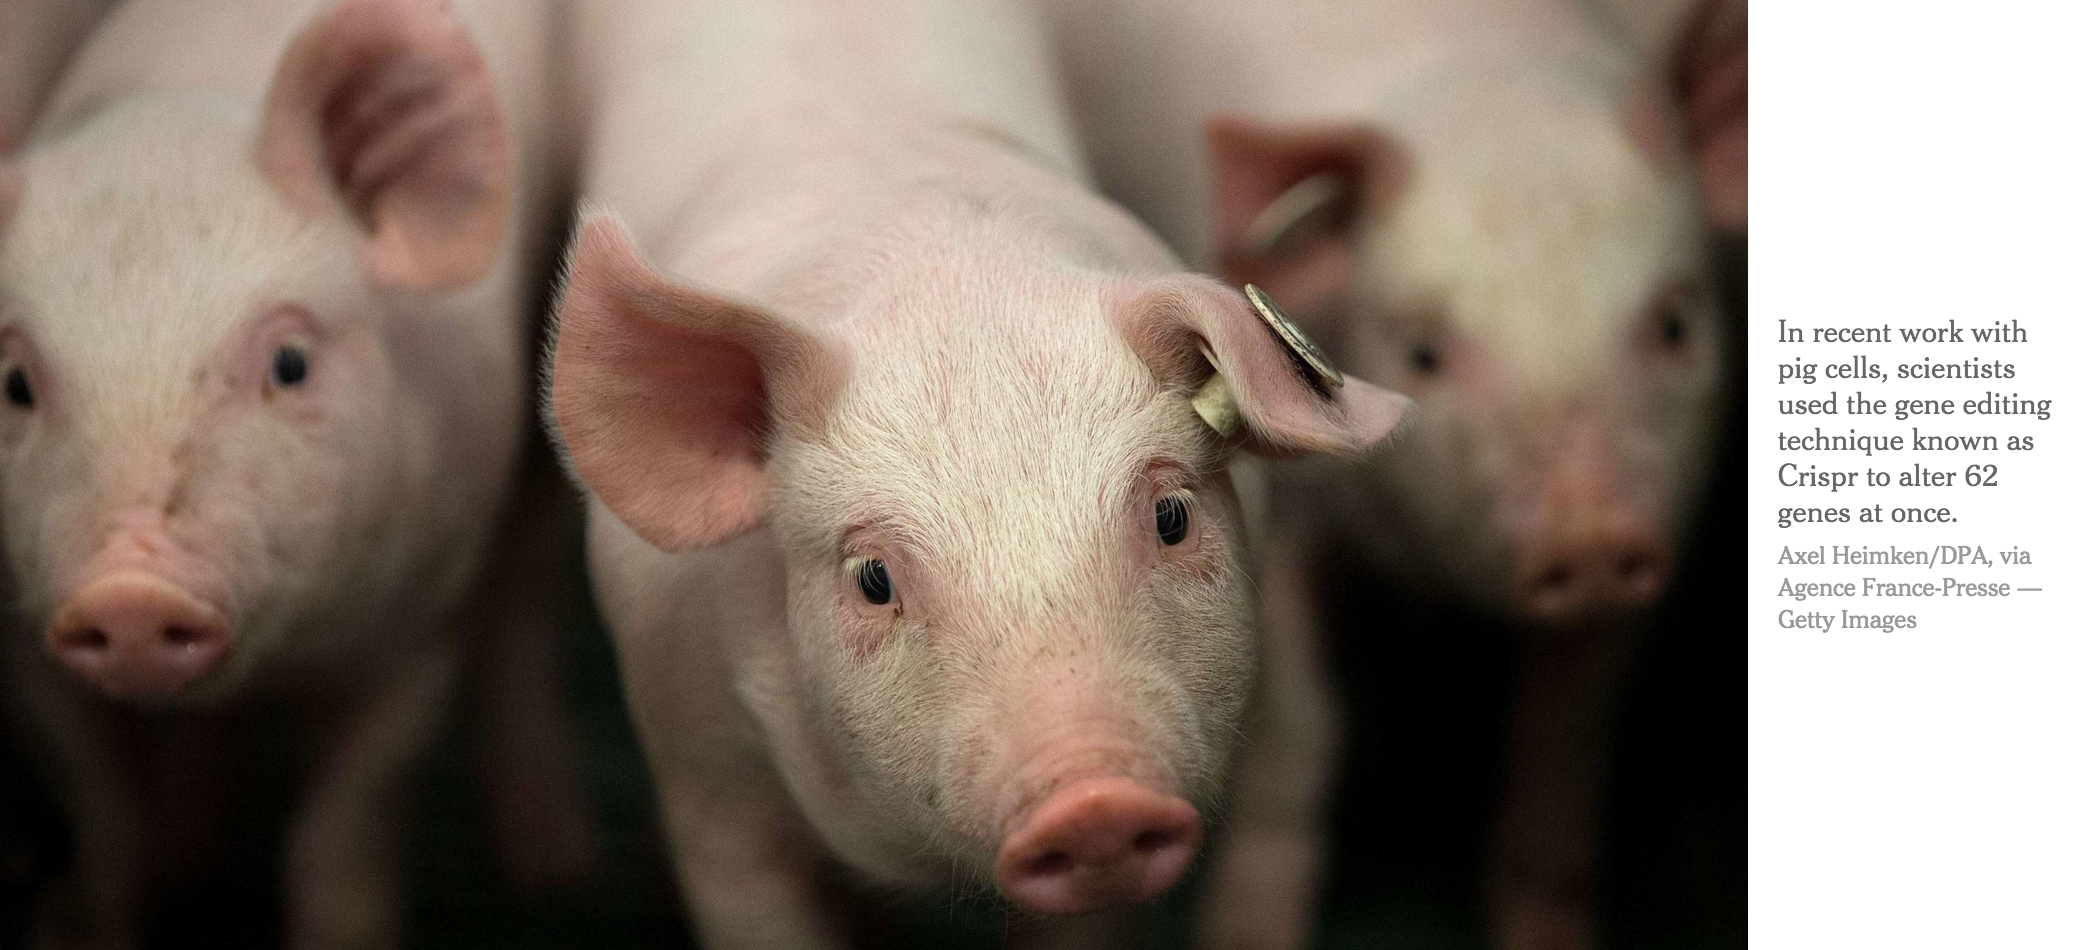
\includegraphics[width=1\textwidth]{edit-pigs.png}
\end{figure}
\end{frame}

\begin{frame}
\frametitle{Genetics meets Surgical Technologies: \\
CRISPR and Xeno-transplantion}
\begin{itemize}
\item CRSIPR : A recently developed method for 
``editing genes.``
\item Xeno-transplantation :
The transplantation of living cells, tissues or organs
from one species to another. 
\item It has been recently shown that a particular
complication that arises in
xeno-transplation, using pig organs,
can be solved through gene-editing via CRISPR. 
\end{itemize}
\end{frame}

\begin{frame}
\frametitle{What happened with CRISPR?}
\begin{itemize}
\item In October of 2015, scientists gathered at the National Academy of Sciences
in Washington to talk about Crispr, a new method for editing genes.

\item Carl Zimmer claims that "In the past couple of years, 
the technique has become so powerful and accessible that many experts are 
calling for limits on its potential uses — especially altering human 
embryos with changes that could be inherited by future generations."
\end{itemize}
\end{frame}
\begin{frame}

\frametitle{CRISPR: a new method for editing genes}
\begin{itemize}
\item 
\end{itemize}
\end{frame}


\begin{frame}
\frametitle{Recent development with CRISPR}
\begin{itemize}
\item "In a typical experiment, scientists use Crispr to alter a single gene.
 But in recent work with pig cells, Dr. Church and his colleagues used Crispr
 to alter 62 genes at once. The researchers hope that this achievement may
 someday make it possible to use pig organs for transplantation into humans." 
(Carl Zimmer) 
\item "But despite the large number of genes involved, 
Dr. Weiss and other experts cautioned that the 
new work doesn’t mean that we’ve suddenly gained the power to 
bypass evolution. Crispr does not allow scientists to manipulate 
genes on a huge scale — yet."

\end{itemize}
\end{frame}

\begin{frame}
\frametitle{Complications of Xeno-plantation with Pig Organs}
\begin{itemize}
\item
In the 1990s, xenotransplantation, a technique that uses pig organs in humans, has been topic much discussed by scientists. They have hoped that the organs from the pigs could be cleaned from the harmful viruses and pathogens that would enter the human host and ultimately harm them. 
\item
However, the issues with this is that in the pig’s DNA there are viral genes. These genes are called endogenous retroviruses; which humans also have. 
\item
The one found in pigs (PERVs) can produce viruses that infect other pig cells. Unfortunately, when mixed with human cells, they are also infected. 
\end{itemize}
\end{frame}


\begin{frame}
\frametitle{Gene-editing Solution to the Complications}
\begin{itemize}
\item
This road block seamed impossible to get rid off to scientists because they were part of the pig’s genome. 
\item
However, Dr. Church was able to figure out a method to disable the PERVs. They started off by finding out there are 62 PERVs found in each cell, and that the PERVs had almost identical DNA. 
\item
What Dr. Church did was design a new set of genes and place them into the pig cells. These new genes created enzymes would find the PERVs and cut them out from the DNA. Within two weeks, the pig cells had changed all the viral DNA. 
\item
Dr. Church was able to accomplish this by creating only one molecule, not 62, to alter the 62 genes.
\end{itemize}
\end{frame}

\end{document}
